\documentclass[12pt,journal,compsoc]{IEEEtran}

\newcommand{\subparagraph}{}

\usepackage[compact]{titlesec}
\titlespacing{\section}{0pt}{1ex}{1ex}
\titlespacing{\subsection}{0pt}{1ex}{0.5ex}
\titlespacing{\subsubsection}{0pt}{0.5ex}{0ex}

\usepackage{graphicx}
\graphicspath{ {../src/img/} }
 
\begin{document}
%
% paper title
% can use linebreaks \\ within to get better formatting as desired
% Do not put math or special symbols in the title.
\title{Assignment 1}

\author{Manas~Joshi,
        Shubham~Singla,
        and~Harsh~Kumar}% <-this % stops a space


% make the title area
\maketitle

\section{Introduction}
\IEEEPARstart{F}{ollowing} report contains observation for the $3$ data sets provided in the assignment namely, FMNIST, Medical data and Railway data. The observations contain the performance of different machine learning algorithms on the above mentioned data sets. The algorithms implemented are PCA, K-Means, KNN, Bayes and Naive Bayes classifier with different class conditional densities namely GMM, Multinomial, Multivariate Normal and Parzen window. Results have been summarized below in the form of accuracy, precision, recall, f-score, micro and macro average precision, recall and f-score.

\section{Medical Data}
\noindent Each of 'Healthy', 'Surgery' and 'Medication' are assigned a number $0$, $1$ and $2$ respectively. Thus, it reduces to a problem of having labeled data with $3$ classes and $3$ features for each data point. The data was observed in 3D and 2D using PCA. Standardization of data followed by a 75/25 split into train and dev set was done. KNN, Bayes and Naive-Bayes Classifier with different class conditional densities as GMM, Multivariate Normal and Parzen Window for Supervised Learning and K-Means clustering for Unsupervised Learning were applied.
\begin{center}
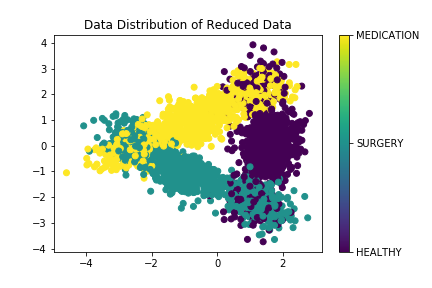
\includegraphics[scale=0.35]{2d_medical.png}

{\small Fig. 1 Visualization of Data in 2D}
\end{center}

\subsection{Observations}
\noindent In all the below tables, F(C$i$) denotes the F-Score for class $i$. Comp. denotes the number of components used in Gaussian Mixture Models (GMM). Vol. denotes the volume parzen window with HC being Hypercube and G being Gaussian kernels. Cf-Type is the type of classifier where B(GMM) denotes Bayes Classifier with class conditional density as GMM, NB(Pz) denotes Naive Bayes classifier with class conditional density as Parzen Window Estimation and MN denotes multinormal. Param. denotes the parameters of the corresponding classifier and class conditional density. Acc. denotes the accuracy.

\noindent In unsupervised learning results, Ngh. denotes the neighbours and M.P. denotes the Minkowski parameter of KNN. In the K-Means result, Iter. denotes the iteration used in K-Means.
\vspace*{0.2 cm}
\subsubsection{Supervised Learning Algorithms}
\vspace*{0.2 cm}

\begin{center}
\begin{tabular}{|c|c|c|c|c|}
\multicolumn{5}{c}{Bayes Classifier - GMM (Dev Set)}\\
\hline
Comp. & Accuracy & F(C1) & F(C2) & F(C3)\\
\hline
$2$ &$0.916$ &$0.9424$ &$0.9171$ &$0.8875$\\
\hline
$3$ &$0.9187$ &$0.9424$ &$0.9199$ &$0.8931$\\
\hline
$4$ &$0.9187$ &$9463$ &$.9174$ &$0.8917$\\
\hline
$5$ &$0.9187$ &$0.9465$ &$0.9165$ &$0.8926$\\
\hline
\end{tabular}
\\
\vspace*{0.2cm}

\begin{tabular}{|c|c|c|c|c|}
\multicolumn{5}{c}{Bayes - Parzen Window (Dev Set)}\\
\hline
Vol & Acc. & F(C1) & F(C2) & F(C3)\\
\hline
$HC(0.5)$ &$0.9013$ &$0.9196$ &$9068$ &$8753$\\
\hline
$HC(1)$ &$0.884$ &$0.913$ &$0.8919$ &$0.8446$\\
\hline
$G(0.5)$ &$0.8787$ &$0.9107$ &$0.8855$ &$0.8377$\\
\hline
$G(1)$ &$0.844$ &$0.9087$ &$0.833$ &$0.7897$\\
\hline
\end{tabular}
\\
\vspace*{0.2 cm}

\begin{tabular}{|c|c|c|c|c|}
\multicolumn{5}{c}{Naive Bayes Classifier - GMM (Dev Set)}\\
\hline
Comp. & Accuracy & F(C1) & F(C2) & F(C3)\\
\hline
$2$ &$0.9213$ &$0.9491$ &$0.9225$ &$0.8908$\\
\hline
$3$ &$0.9213$ &$0.9474$ &$0.9225$ &$0.8922$\\
\hline
$4$ &$0.92$ &$0.9455$ &$0.9245$ &$0.8874$\\
\hline
$5$ &$0.913$ &$0.9379$ &$9145$ &$0.8855$\\
\hline
\end{tabular}

\vspace*{0.2 cm}

\begin{tabular}{|c|c|c|c|c|}
\multicolumn{5}{c}{N. Bayes - Parzen Window (Dev Set)}\\
\hline
Vol & Acc. & F(C1) & F(C2) & F(C3)\\
\hline
$HC(0.5)$ &$0.9$ &$0.9311$ &$0.9009$ &$0.867$\\
\hline
$HC(1)$ &$0.8853$ &$0.927$ &$0.8845$ &$0.845$\\
\hline
$G(0.5)$ &$0.872$ &$0.9195$ &$0.875$ &$0.8205$\\
\hline
$G(1)$ &$0.792$ &$0.8512$ &$0.7469$ &$0.7721$\\
\hline
\end{tabular}

\vspace*{0.2 cm}
\begin{table*}
\centering
\begin{tabular}{|c|c|c|c|c|c|}
\multicolumn{6}{c}{Classifier with Best Parameters on Medical Test Data}\\
\hline
Cf-Type & Para. & Acc. & F(C1) & F(C2) & F(C3)\\
\hline
B(GMM) &$4$ &$0.9$ &$0.9276$ &$0.8824$ &$0.8916$\\
\hline
B(Pz) &G(0.25) &$0.888$ &$0.9159$ &$0.8784$ &$0.8722$\\
\hline
B(MN) &- &$0.5027$ &$6251$ &$0.4137$ &$0.3976$\\
\hline
NB(GMM) &$3$ &$0.899$ &$0.9277$ &$0.8822$ &$0.8884$ \\
\hline
NB(Pz) &$HC(0.5)$ &$0.8927$ &$0.9216$ &$0.8801$ &$0.878$\\
\hline
\end{tabular}
\end{table*}

\vspace*{0.2 cm}
\begin{tabular}{|c|c|c|c|c|c|}
\multicolumn{6}{c}{KNN on 3D Data Set (Dev Set)}\\
\hline
Ngh. & M.P. & Acc. & F(C1) & F(C2) & F(C3)\\
\hline
$1$ &$2$ &$0.8733$ &$0.9047$ &$0.8636$ &$0.8517$\\
\hline
$5$ &$2$ &$0.904$ &$0.9246$ &$0.9$ &$0.887$\\
\hline
$10$ &$2$ &$0.9107$ &$0.9284$ &$0.9091$ &$0.8937$\\
\hline
$15$ &$2$ &$0.916$ &$0.9286$ &$0.922$ &$0.8964$\\
\hline
$1$ &$inf$ &$0.872$ &$0.9087$ &$0.8582$ &$0.8493$\\
\hline
$5$ &$inf$ &$0.8933$ &$0.9187$ &$0.8831$ &$0.8785$\\
\hline
$10$ &$inf$ &$0.908$ &$0.9218$ &$0.9091$ &$0.8922$\\
\hline
$15$ &$inf$ &$0.9133$ &$0.926$ &$0.917$ &$0.8964$\\
\hline
$1$ &$$-$inf$ &$0.6333$ &$0.6613$ &$0.6463$ &$0.59$\\
\hline
$5$ &$$-$inf$ &$0.7627$ &$0.7992$ &$0.7416$ &$0.7441$\\
\hline
$10$ &$$-$inf$ &$0.82$ &$0.8523$ &$0.8031$ &$0.8017$\\
\hline
$15$ &$$-$inf$ &$0.8373$ &$0.8598$ &$0.8111$ &$0.8398$\\
\hline
\end{tabular}


\end{center}
KNN on $3$ dimensional data with $5$ neighbors and Euclidean distance performed best.\\
Performance on test data1-\\ 
Accuracy - $0.8843$\\ F-Score (Class 1) - $0.9169$\\
F-Score (Class 2) - $0.8654$\\ F-Score (Class 3) - $0.8725$\\ Macro Average F-Score - $0.8858$\\
Micro Average F-Score - $0.8843$\\
KNN was run on 2D dataset obtained after PCA, but the performance decreased. Hence, further analysis was not done on 2D data.
\subsubsection{Unsupervised Learning Algorithm}
\vspace*{0.1 cm}
\begin{center}
\begin{tabular}{|c|c|c|c|c|}
\multicolumn{5}{c}{K-Means (Test Set)}\\
\hline
Iter. & Accuracy & F(C1) & F(C2) & F(C3)\\
\hline
$40$ &$0.57$ &$0.4593$ &$0.5835$ &$0.4214$\\
\hline
$80$ &$0.65$ &$0.6593$ &$0.5312$ &$0.5871$\\
\hline
\end{tabular}
\end{center}
\subsection{Conclusion}
\noindent Maximum accuracy od $0.9$ for Bayes classifier is obtained using a Gaussian Mixture model with 4 components. For Parzen window density estimation accuracy increases as the size of window decreases. Very small values were not chosen to avoid empty volumes. Assuming Gaussian window with cube length of $0.25$, accuracy of 0.888 was obtained. It increases slightly in case of Naive Bayes to $0.8927$ using a hypercube with cube length of 0.5. For Multivaraite Normal class conditional distribution, bayes classifier gives an accuracy of $0.5027$. KNN also gives a high accuracy of 0.8843 considering 5 neighbours using Euclidean distance. It was also observed that on applying PCA and reducing the data to 2 dimensions resulted in decrease in the accuracy. 
\section{Railway Data}
\noindent The labels corresponding to each data point were in binary format denoting BOARDED AND NON-BOARDED CASES. The discrete features in the Railway data included the sex column and Prefered class column. Both of them were encoded first with female as $1$ and male as $0$ in the sex column and $FIRST_AC$ as $1$, $SECOND_AC$ as $2$, $THIRD_AC$ as $3$ and $NO_PREF$ as $0$. Different Machine Learning models were tested first on this encoding. Later the sex and prefered class feature columns were encoded using one-hot encoding with the prefered column converted to three distinct columns for first, second and third class leaving the no pref case for statistical independence. 

\begin{enumerate}
\item Using PCA to visualize the data in 2 dimensions.

\item Splitting the dataset using the data utils helper module to divide the entire dataset into three parts. Train: Test: Validation=0.8:0.1:0.1

\end{enumerate}
\pagebreak
\subsection{Observations}
\subsubsection{Supervised Learning Algorithms}
\begin{center}
\begin{tabular}{|c|c|c|c|c|}
\multicolumn{5}{c}{Bayes Classifier - GMM (Railway Dev Set)}\\
\hline
Comp. & Accuracy & F(C1) & F(C2) & Micro F\\
\hline
$2$ &$0.716$ &$0.5024$ &$0.8071$ &$0.7175$ \\
\hline
$3$ &$0.7387$ &$0.5724$ &$0.8099$ &$0.7331$ \\
\hline
$4$ &$0.7387$ &$0.5763$ &$.8074$ &$0.7317$ \\
\hline
$5$ &$0.7387$ &$0.5763$ &$.8074$ &$0.7317$ \\
\hline
\end{tabular}
\newline

\begin{tabular}{|c|c|c|c|c|}
\multicolumn{5}{c}{Best Classifier on Railway Test Data}\\
\hline
Cf-Type & Para. & Acc. & F(C1) & F(C2) \\
\hline
B(GMM) &$3$ &$0.79$ &$0.6976$ &$0.8124$ \\
\hline
B(MN) &- &$0.698$ &$0.5759$ &$0.7684$ \\
\hline
B(PCA) &- &$0.5727$ &$0.3462$ &$0.7237$ \\
\hline
NB(GMM) &$1$ &$0.649$ &$0.6477$ &$0.7822$  \\
\hline
NB(mix) &$-$ &$0.7127$ &$0.6216$ &$0.7601$ \\
\hline
\end{tabular}

\begin{tabular}{|c|c|c|c|c|}
\multicolumn{5}{c}{KNN on one-hot Data Set (Dev Set)}\\
\hline
Ngh. & M.P. & Acc. & F(C1) & F(C2) \\
\hline
$1$ &$1$ &$0.7033$ &$0.6047$ &$0.7636$ \\
\hline
$5$ &$1$ &$0.724$ &$0.6246$ &$0.78$\\
\hline
$10$ &$1$ &$0.7307$ &$0.6484$ &$0.7891$ \\
\hline
$15$ &$1$ &$0.746$ &$0.6486$ &$0.792$ \\
\hline
$1$ &$2$ &$0.692$ &$0.5987$ &$0.7582$ \\
\hline
$5$ &$2$ &$0.7133$ &$0.6087$ &$0.7831$ \\
\hline
$10$ &$2$ &$0.728$ &$0.6418$ &$0.7791$ \\
\hline
$15$ &$2$ &$0.7333$ &$0.616$ &$0.7917$ \\
\hline
$1$ &$3$ &$0.7433$ &$0.6113$ &$0.8063$ \\
\hline
$5$ &$3$ &$0.7227$ &$0.6092$ &$0.7816$ \\
\hline
$10$ &$3$ &$0.72$ &$0.6323$ &$0.6831$ \\
\hline
$15$ &$3$ &$0.7373$ &$0.6298$ &$0.7911$ \\
\hline
\end{tabular}
\end{center}

\noindent Using Bayes Classifier after reducing dimesnions such that percent variance retained is 99 resulted in drop of 20 percent in accuracy. 

\subsubsection{Unsupervised Learning Algorithms}

\noindent K-means Clustering gives poor predictions as the euclidean distance kernel is not a good measure. Kmeans Accuracy on Dev Set =  49.5419

\pagebreak
\subsection{Conclusion}
\noindent Bayes classifier with gaussian mixture model of 3 components gives best accuracy of  $79$ percent on test data. KNN classifier gives a reasonable performance with about $77$ percent test accuracy with $15$ neighbours and Minkowski Parameter = 1. The K Means Clustering algorithms using euclidean distance as kernel fails badly which suggest that eucleadean distance does not hold any good similarity between data points. One thing that is confusing is that though the features fairly seem independent of each other, the naive bayes failed to improve the accuracy significantly. One of reasons maybe poor MLE estimate of multinomial distribution and also the hyperparameters in bayesian estimation for the prior districution effect the results greatly. Another interesting phenomenon observed in this dataset is that even though PCA captures 99 percent of the variance explained by the data, the training on transformed data causes the accuracy of mixture modeled bayes classifier to drop drastically by almost 20 percent. This may be because of the under lying non linear relationships between the feature spaces which are not captured by PCA. Overall the bayesian decision models doesn’t appear to work very significantly on discrete categorical feature spaces.
\section{FASHION MNIST Data}
\noindent This is a multi class classification problem where the feature vectors are sparse. Constrained by the memory and computational power, the number of experiments for this dataset were reduced. Standardizing the dataset with each feature having zero mean and unit variance resulted in unsatisfactory results. Therefore, another normalization technique was used where each example was scaled to have unit norm. Here, rather than performing validation (computationally expensive) on a split of training dataset, the best parameters were chosen based on prediction on test data. The dimensionality of dataset was reduced to 25 and 5. Bayes Classifier with GMM, Multivariate Normal MLE and Parzen class conditional density, Naive-Bayes classifier with Gaussian MLE and KNN was used for Supervised Learning. K-Means Clustering was used as an Unsupervised Learning method.
\subsection{Observations}
\noindent We use the same nomenclature as previously mentioned. 

\noindent Here, Dim. refers to the dimension of data after PCA has run on it. Macro-F refers to the Macro average for F score of all classes and similarily, Micro-F refers to the Micro average for F score of all classes
\subsubsection{Supervised Learning Algorithms}

\begin{center}
\begin{tabular}{|c|c|c|c|c|}
\multicolumn{5}{c}{Bayes Classifier - GMM (Test Set)}\\
\hline
Dim. & Comp. & Acc. & Macro-F & Micro-F\\
\hline
$25$ &$2$ &$0.8194$ &$0.8179$ &$0.8194$\\
\hline
$25$ &$4$ &$ 0.8319$ &$0.8311$ &$0.8319$\\
\hline
$5$ &$2$ &$0.707$ &$0.7042$ &$0.7070$\\
\hline
$5$ &$4$ &$ 0.7211$ &$0.7203$ &$0.7211$\\
\hline
\end{tabular}
\vspace{0.4cm}

\begin{tabular}{|c|c|c|c|c|}
\multicolumn{5}{c}{Bayes Classifier - Parzen Window (Test Set)}\\
\hline
Dim. & Vol & Acc. & Macro-F & Micro-F\\
\hline
$25$ &$HC(0.1)$ &$0.6095$ &$0.7013$ &$0.6095$\\
\hline
$25$ &$HC(0.25)$ &$ 0.7754$ &$0.779$ &$0.7754$\\
\hline
$25$ &$G(0.1)$ &$ 0.809$ &$0.8122$ &$0.809$\\
\hline
$25$ &$G(0.25)$ &$ 0.7062$ &$0.7212$ &$0.7062$\\
\hline
$5$ &$HC(0.1)$ &$0.7374$ &$0.7379$ &$0.7374$\\
\hline
$5$ &$HC(0.25)$ &$ 0.6679$ &$0.6	683$ &$0.6679$\\
\hline
$5$ &$G(0.1)$ &$0.6636$ &$0.6643$ &$0.6636$\\
\hline
$5$ &$G(0.25)$ &$0.6023$ &$0.5947$ &$0.6023$\\
\hline
\end{tabular}
\vspace*{0.4 cm}

\begin{tabular}{|c|c|c|c|c|}
\multicolumn{4}{c}{Bayes Classifier - Normal MLE (Test Set)}\\
\hline
Dim. & Acc. & Macro-F & Micro-F\\
\hline
$50$ &$0.8188$ &$0.8191$ &$0.8188$\\
\hline
$25$ &$0.8064$ &$0.8053$ &$0.8064$\\
\hline
$5$ &$0.6872$ &$0.6833$ &$0.6872$\\
\hline
\end{tabular}
\vspace{0.2cm}

\begin{tabular}{|c|c|c|c|c|c|}
\multicolumn{6}{c}{KNN (Test Set)}\\
\hline
Dim. & Ngh. & M.P. & Acc. & Macro-F & Micro-F\\
\hline
$25$ &$5$ &$1$ &$0.8568$ &$0.8568$ &$0.8568$\\
\hline
$25$ &$5$ &$2$ &$0.8576$ &$0.8575$ &$0.8576$\\
\hline
$25$ &$10$ &$2$ &$0.8589$ &$0.8587$ &$0.8589$\\
\hline
$25$ &$5$ &$inf$ &$0.8474$ &$0.8472$ &$0.8474$\\
\hline
$5$ &$5$ &$1$ &$0.7379$ &$0.7366$ &$0.7379$\\
\hline
$5$ &$5$ &$2$ &$0.7327$ &$0.7311$ &$0.7327$\\
\hline
$5$ &$10$ &$2$ &$0.7449$ &$0.7435$ &$0.7449$\\
\hline
$5$ &$5$ &$inf$ &$0.7352$ &$0.7341$ &$0.7352$\\
\hline
\end{tabular}
\end{center}
KNN $5$ neighbors and Euclidean distance performed best.\\
Performance on test data:\\ 
Accuracy - $0.8576$\\ Macro Average F-Score - $0.8575$\\
Micro Average F-Score - $0.8576$
\subsection{Conclusion}
\noindent Maximum accuracy of $0.8319$ for Bayes classifier is obtained using a Gaussian Mixture model with 4 components and data of dimensionality 25. For Parzen window density estimation accuracy increases as the size of window decreases. Very small values were not chosen to avoid empty volumes. Assuming Gaussian window with cube length of $0.1$, accuracy of 0.809 was obtained. For Multivaraite Normal class conditional distribution, bayes classifier gives an accuracy of $0.8188$ with dimensions reduced to 50. KNN also gives a high accuracy of 0.8589 considering 10 neighbours and using euclidean distance as the distance metric. 

\subsection{References}

\noindent [1] The EM Algorithm. Retrieved from https://www.ics.uci.edu/~smyth/courses/cs274/
notes/EMnotes.pdf\\
\noindent [2] Fashion MNIST Reader. Retrieved from https://github.com/zalandoresearch/fashion-mnist/blob/master/utils/mnist\_reader.py\\
\noindent [3] Regularization in GMM. Retrieved from https://stats.stackexchange.com/questions/
35515/matlab-gmdistribution-fit-regularize-what-regularization-method\\
\noindent [4] Metric for multiclass classification. Retrieved from https://stats.stackexchange.com
/questions/51296/how-do-you-calculate-precision-and-recall-for-multiclass-classification-using-co

\end{document}


